\documentclass{standalone}
\usepackage{tikz}
\usepackage{ctex,siunitx}
\setCJKmainfont{Noto Serif CJK SC}
\usepackage{tkz-euclide}
\usepackage{amsmath}
\usetikzlibrary{patterns, calc,3d}
\usetikzlibrary {decorations.pathmorphing,decorations.pathreplacing,decorations.shapes}
\tikzset{label style/.append style={font=\small}}
\begin{document}
\small
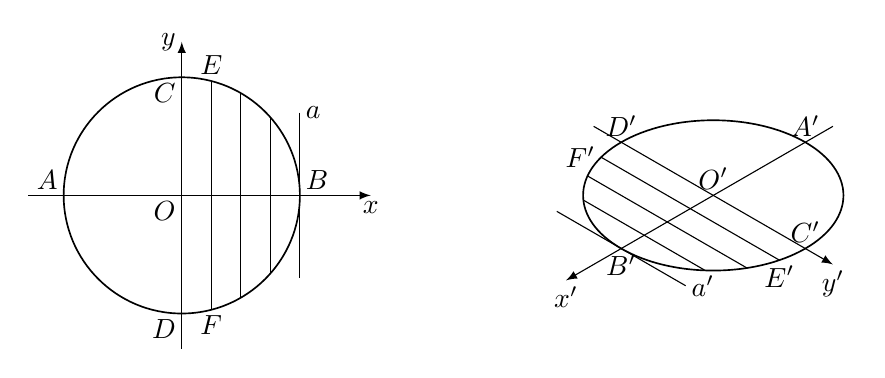
\begin{tikzpicture}[>=latex,scale=1.5,inner sep=2pt]
\begin{scope}
  \draw[->](-1.3,0)--(1.6,0)node[below]{$x$};
  \draw[->](0,-1.3)--(0,1.3)node[left]{$y$};
  \draw[semithick](0,0)node[below left]{$O$}circle(1);
  \foreach \x in {1,2,3}
  {\draw ({\x/4},{-sqrt(1-\x*\x/16)})--({\x/4},{sqrt(1-\x*\x/16)});}
  \node at (0.25,{sqrt(15)/4})[above]{$E$};
  \node at (0.25,{-sqrt(15)/4})[below]{$F$};
  \node at (0,-1)[below left]{$D$};
  \node at (0,1)[below left]{$C$};
  \node at (-1,0)[above left]{$A$};
  \node at (1,0)[above right]{$B$};
  \draw (1,0.7)node[right]{$a$}--(1,-0.7);
\end{scope}
\begin{scope}[xshift=4.5cm,x={(-150:9mm)},z={(-30:9mm)},canvas is xz plane at y=0]
  \draw[->](-1.3,0)--(1.6,0)node[below]{$x'$};
  \draw[->](0,-1.3)--(0,1.3)node[below]{$y'$};
  \draw[semithick](0,0)node[above]{$O'$}circle(1);
  \foreach \x in {1,2,3}
  {\draw ({\x/4},{-sqrt(1-\x*\x/16)})--({\x/4},{sqrt(1-\x*\x/16)});}
  \node at (0.25,{sqrt(15)/4})[below]{$E'$};
  \node at (0.25,{-sqrt(15)/4})[left]{$F'$};
  \node at (0,-1)[above]{$D'$};
  \node at (0,1)[above]{$C'$};
  \node at (-1,0)[above]{$A'$};
  \node at (1,0)[below]{$B'$};
  \draw (1,0.7)node[right]{$a'$}--(1,-0.7);
\end{scope}
\end{tikzpicture}
\end{document}